
\documentclass[11pt]{article}

\usepackage{amsmath} %import amsmath for align command
\usepackage{cite} %import package for using bibtex bibliography
\usepackage{graphicx} %import package for inserting figures from image files
\usepackage{mathtools} %import package for using certain symbols such as eq. arrows
\usepackage{tikz} %import package for creating figures
\usepackage{booktabs}
\usepackage{siunitx}
\usepackage[T1]{fontenc}
\usepackage[font=small,skip=0pt]{caption}


\usepackage{placeins}
\usepackage{array}
\newcolumntype{P}[1]{>{\centering\arraybackslash}p{#1}}

\usepackage[nodisplayskipstretch]{setspace}


\usepackage{titlesec}
\titlespacing{\section}{0pt}{0.8\baselineskip}{0.8\baselineskip}
\titlespacing{\subsection}{0pt}{0.675\baselineskip}{0.675\baselineskip}
\setlength{\abovecaptionskip}{2pt plus 2pt minus 5pt}

% for referencing links
\usepackage{hyperref}
\hypersetup{
	colorlinks=true,
	linkcolor=blue,
	filecolor=magenta,
	urlcolor=cyan,
}

% \usepackage{apacite}

\usepackage{algorithm}
\usepackage[noend]{algpseudocode}
\usepackage{textcomp}
\usepackage{subcaption}

%change default margins
\setlength{\topmargin}{-.75in}
\setlength{\textheight}{9.5in}

\setlength{\oddsidemargin}{0in}
\setlength{\evensidemargin}{0in}
\setlength{\textwidth}{6.6in}

\graphicspath{{aima/images/}}

\newcommand{\urlNewWindow}[1]{\href[pdfnewwindow=true]{#1}{\nolinkurl{#1}}}
\newcommand{\problemone}{grid world problem}
\newcommand{\Problemone}{grid world problem}
\newcommand{\problemtwo}{choice suggestion problem}
\newcommand{\Problemtwo}{choice suggestion problem}
\newcommand{\expnumber}[2]{{#1}\mathrm{e}{#2}}

\begin{document}

%create title
\title{Deep Reinforcement Learning Nanodegree\\
	   Project 1 -- Navigation Report}
\author{\vspace{-1mm}Chris Cadonic\\
chriscadonic@gmail.com}
\maketitle
\vspace{-1.5em}

\section{Introduction}

As part of the first project for the deep reinforcement learning nanodegree, I built and trained an agent that learns how to navigate through a world with yellow and blue bananas in an effort to maximize how many yellow bananas it can acquire.

\subsection{Environment Overview}

In the Unity-ML environment provided, the agent navigates through a world filled with yellow and blue bananas. As the agent moves through the world, if it comes into contact with a banana it will pick it up, receiving a reward of +1 if it picks up a yellow banana and -1 if it picks up a blue banana. Its goal is to maximize its reward for a single play session where it navigates and tries to pick up as many yellow bananas while avoiding blue bananas. The game is considered solved if it achieves an average score of \textbf{+13} over 100 games.

As the agent interacts, it receives information from the environment of the form of a 37-value vector containing information about the agents velocity, and ray projections informing the agent about objects in front of its current position.


\FloatBarrier

\begin{figure}[!ht]
	\centering
	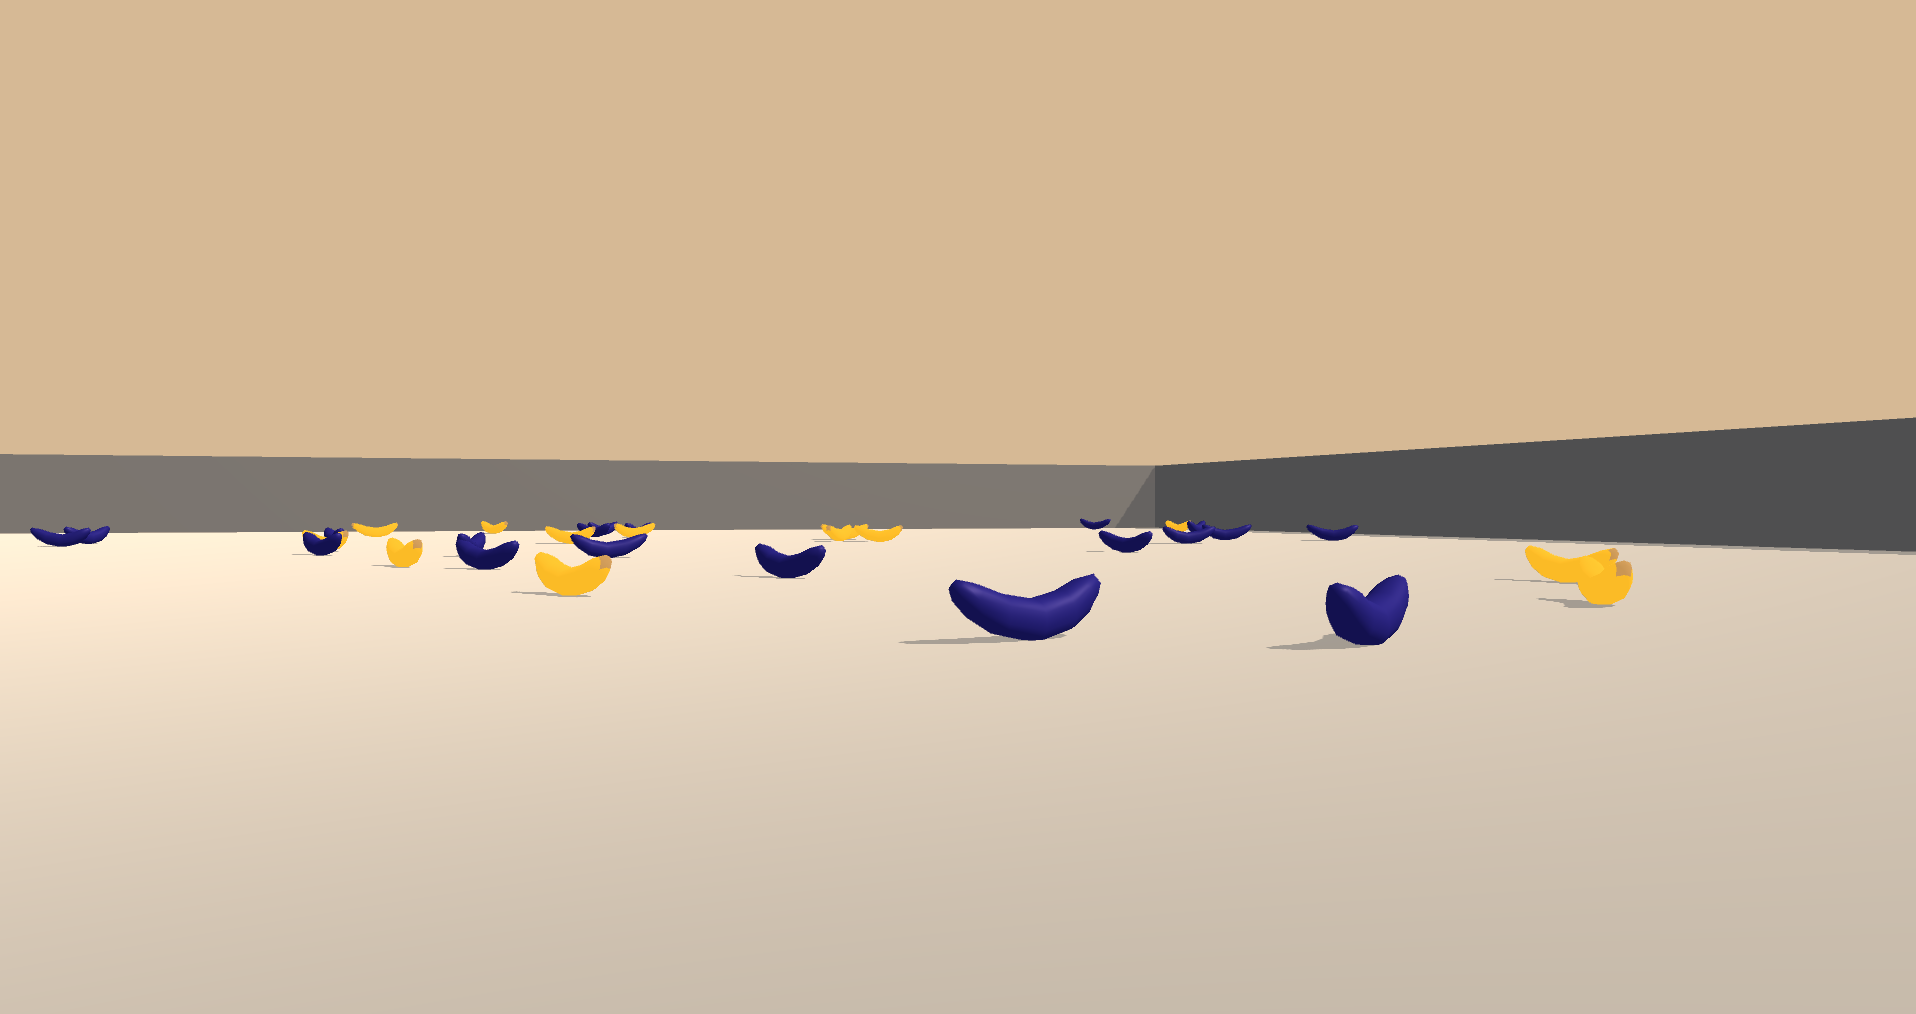
\includegraphics[width=0.75\linewidth]{images/example-game-image.png}
	\caption{A snapshot of the banana navigation game.}
	\label{fig:example-game-image}
\end{figure}

\FloatBarrier

Interactions available to the agent include moving in one of four directions:
\begin{itemize}
	\item move forward,
	\item move backward,
	\item turn left,
	\item turn right,
\end{itemize}
with these four actions forming the action space $\mathcal{A}$. The agent solves the game by understanding what the optimal action is to take in each of the possible states that it finds itself in. An example image of the game is shown in Fig. \ref{fig:example-game-image}.


\section{Approach}

Initially I had approached this problem by first attempting to use Q-learning as
a first benchmark, but given the continuous nature of the state space
$\mathcal{S}$ this would also necessitate discretization or tile coding the
space. For this reason, I instead chose to implement a vanilla DQN (Deep
Q-network) and iteratively improve it to achieve better performance.

\subsection{DQN}

The DQN algorithm extends the capabilities of Q-learning algorithms by leveraging deep neural networks to approximate the optimal action-value function $q_*(s, a)$. That is, how much expected reward is associated with taking an action $a$ while in state $s$. 

To do this, the input layers of the neural network take in the state-vector represented by the environment, which enables continuous values for each state feature. This is the case in the current navigation problem. Furthermore, the neural network must then also contain a layer of output units that correspond to the different actions available, which is a discrete space of 4 options, thus enabling us to map states to action values. Thus, the agent uses gradient descent to learn from experience tuples to update the network weights $\theta$ such that it can better approximate action values for a provided state vector.

Some key alterations to the general Q-learning algorithm that enable a neural network to stably and reliably learn an estimate of the action-value function $\hat{q}(s, a)$ were implemented in the current work.

The first alteration is the use of a \textit{replay buffer}, which maintains a long-term size-limited storage of experience tuples. This is used by providing randomly sampled batches of experience tuples for the agent to learn from, rather than learning from experience tuples as they arrive, in order to minimize the effect of temporal correlation between experience tuples that the agent learns from back-to-back.

Secondly, using a \textit{pair} of identically constructed neural networks, labelled $Q_{target}$ and $Q_{network}$, where the $Q_{network}$ is the primary network used for training and current value estimation, and the $Q_{target}$ is semi-fixed so as to enable a more stable TD-target to be compared against during loss calculations. This means that the $Q_{target}$ network is updated more slowly, updating every $m$ iterations to match the $Q_{network}$, so that the $Q_{network}$ is updated not against itself, but against what appears to be a stable action-value approximation.


\subsection{Implementation}

The navigation code implemented takes tuples of the form ($s$, $a$, $r$, $s_{next}$, $done$), where $done$ indicates whether the episode has been completed, and stores these into the replay buffer as the agent interacts with the world. Actions the agent takes are determined by using an $\epsilon$-greedy strategy, where with probability $\epsilon$ it will take a random action and otherwise use the primary Q-network to determine which action it should take. This value starts at a very high value, 1.0 here, to promote early exploration, and decays to a minimum value of $0.05$ over time. Values are extracted from both the primary Q-network and target network by provided a single or batch of states $s$ and determining the output values from the final layer of the networks to extract $q(s, a)$.

When the agent attempts to learn experience tuples randomly sampled from the replay buffer, it uses the following updates:

\begin{equation} \label{eq:update}
	\Delta \theta_{q} = \alpha (r + \gamma \max_{a}{\hat{q}(s_{next}, a, \theta_{target})} - \hat{q}(s, a, \theta_{q}))\nabla_{\theta_{q}}\hat{q}(s, a, \theta_{q})
\end{equation}
where $\theta_{target}$ and $\theta$ represent the target and primary Q-network weights respectively, $\alpha$ is the learning rate or step size parameter, and $\gamma$ is the discount factor for weighing how much the agent should incorporate learning from future rewards compared to current rewards. Using Eq. \ref{eq:update} to train the primary Q-network and using a soft update to slowly transfer weights to the target network using:
\begin{equation}\label{eq:soft-update}
\theta_{target} \leftarrow (1 - \tau)\theta_{target} + \tau\theta_{q}
\end{equation}
where $\tau$ is a parameter for controlling how much of the target network is updated by the primary Q-network. This occurs on the basis of every 100 iterations.

By implementing an experience replay buffer, an abstraction of a Q-network that enables an agent class to maintain both a target Q-network as well as a primary Q-network, and an outer wrapper class for coordinating training and model updates, I was able to implement the DQN algorithm and solve the navigation problem presented. In the DQN algorithm, however, there are a number of parameters that required optimization and/or careful selection in order for the algorithm to properly learn in the environment.

For the architecture, I chose to experiment with a deeper model that leveraged increasingly wider linear layers,
 ending up with an 8-layer neural network with units of sizes [64, 64, 128, 128, 
 256, 256, 512, 512] and $ReLU$ activation functions between each layer. The architecture is shown in Fig. \ref{fig:dqn-architecture}.

 \FloatBarrier
 
 \begin{figure}[!ht]
 	\centering
 	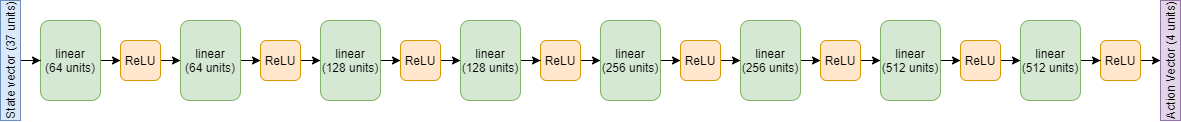
\includegraphics[width=\linewidth]{images/dqn-architecture.png}
 	\caption{The 8-layer MLP used in the DQN algorithm.}
 	\label{fig:dqn-architecture}
 \end{figure}
 
 \FloatBarrier
 
  This architecture was experimented with and ultimately chosen to capture ever-increasingly complex relationships between the state values in the input, determining more high-order information between ray projections as states are passed further into a deeper network.

I also needed to experiment hyperparameter tuning for the following hyperparameters:

\FloatBarrier

\begin{table}[!ht]
	\centering
	\begin{tabular}{ c | c }
	\textbf{hyperparameter} & \textbf{values} \\
	\hline
	$\epsilon_{decay}$ & $[0.99, 0.996, 0.999, 0.9999, 0.99999]$ \\
	$\alpha$ & $[0.00005, 0.0001, 0.0005, 0.001, 0.005]$ \\
	$\tau$ & $[0.005, 0.01, 0.1]$ \\
	$\gamma$ & $[0.8, 0.9, 0.95, 0.99]$ \\
	\hline
	\end{tabular}
	\caption{Hyperparameters experimented with to train an agent using DQN.}
	\label{tbl:hyperparameters}
\end{table}

\FloatBarrier

Even though learning performance from the vanilla DQN was quite good (see results in
Fig. \ref{fig:dqn-results}), I wanted to see explore options to determine if
performance could be improved.
%
%\subsection{Improving DQN}
%
%Since I had the least experience with implementing prioritized experience
%replay, this was the first method I chose to expand on my vanilla DQN.
%
%\subsubsection{Prioritized Experience Replay}
%
%Using prioritized experience replay expands on the idea of sampling from the
%replay buffer to provide experience tuples for the agent to learn from. In the
%original DQN algorithm, this sampling is uniform across all stored experience
%tuples in the replay buffer, whereas prioritized experience replay
%\textit{prioritizes} experience tuples that resulted in a larger loss from
%expected Q-values, capturing that these tuples may have been more impactful
%during the learning process and will likely be more useful to sample more often
%than lesser impactful experience tuples.
%
%In order to expand on my initial implementation, I changed the following:
%- storage of 


\section{Results and Discussion}

\subsection{Learning Performance}

The results in Fig. \ref{fig:dqn-results} show that the the vanilla DQN
algorithm with the architecture shown in Fig. \ref{fig:dqn-architecture} achieved 
quite good performance, solving the navigation problem in 1185 episodes. That is, 
achieving an average score of +13 over 100 episodes after the 1185th episode.

\FloatBarrier

\begin{figure}[!ht]
	\centering
	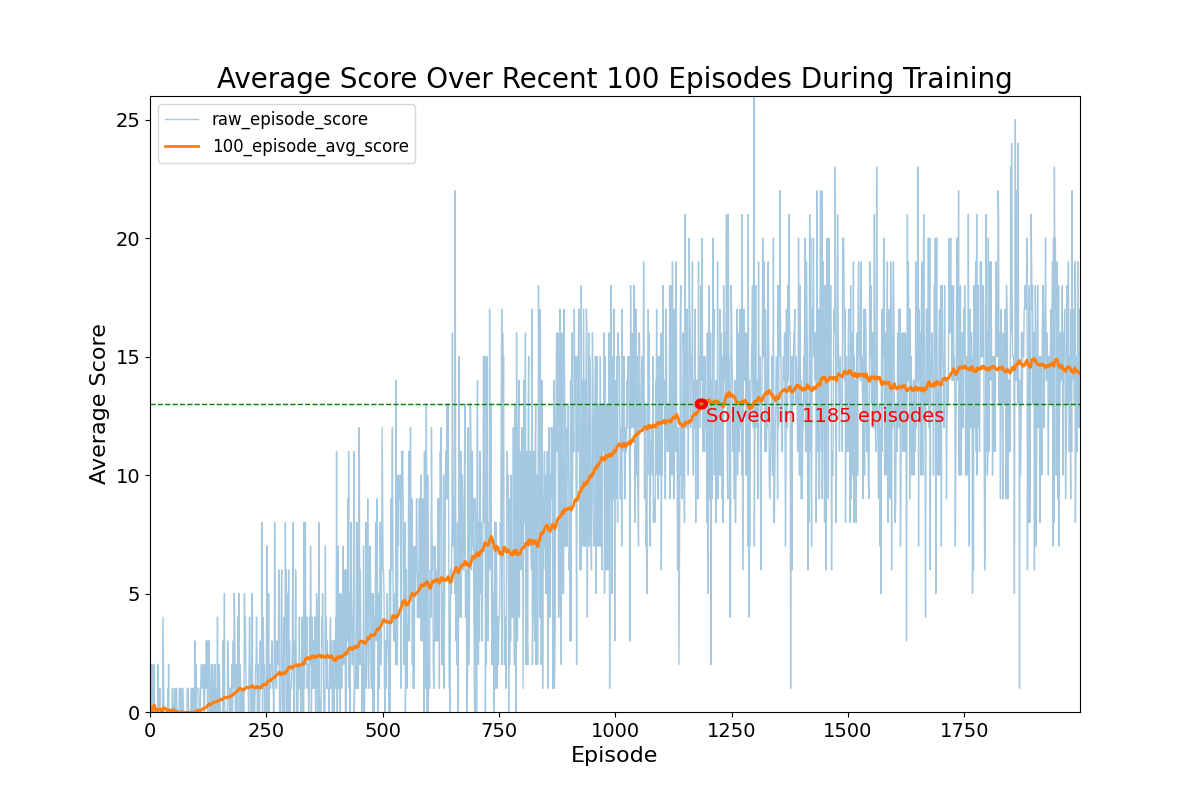
\includegraphics[width=0.9\linewidth]{images/dqn-results.png}
	\caption{}
	\label{fig:dqn-results}
\end{figure}

\FloatBarrier

After running experimentation over the parameters listed in Tbl. \ref{tbl:parameters} 
the optimal parameters were:
\begin{itemize}
	\item $\epsilon_{decay} = 0.996$,
	\item $\alpha = 0.001$,
	\item $\tau = 0.01$,
	\item $\gamma = 0.99$.
\end{itemize}

Evident in the learning performance of the agent, not only was the agent able to 
solve the navigation problem fairly quickly, but it was able to continue to improve 
beyond this, likely because I also enforced a minimum value on $\epsilon_{min} = 0.05$ 
to ensure that the agent is never \textit{entirely} acting greedily.

Although performance tends to improve consistently over the 2000 episode training period, there is quite a bit of variation in the raw episode scores indicated by the light blue line. This is likely due to the aforementioned lower bound of 0.05 on $\epsilon$, which means that the agent still acts completely random 5\% of the time. This lower bound is reached fairly rapidly with $\epsilon_{decay}=0.996$, at approximately episode 747 (i.e., $log_{0.996}(0.05) \approx 747$).

\subsection{Next Steps}


There remains room for improvement for the algorithm, although through experimentation with a vanilla DQN I was able to achieve fairly good results. With regard to experimentation and overall improvement of the DQN algorithm at hand, it may make sense to experiment more with the rate at which the target network is updated a bit more. Currently, the target network is not only updated on a static basis of every 100 iterations, but I also use a soft-update that doesn't completely transfer weights from the Q-network to the target network but rather transfers as in Eq. \ref{eq:soft-update}.

Additionally, it may be interesting to determine if the algorithm may be able to improve if the learning rate $\alpha$ was adaptive rather than static, which may enable the algorithm to learn less and less. This could provide a better overall agent in the end, particularly if $\epsilon$ is decayed to a smaller lower bound, since then the agent could learn from exploration sufficiently well and when it has reached a point that it will no longer be learning much from new actions, it has little to gain from taking completely random actions.

Some logical next steps beyond optimizing vanilla DQN, however, would include:
\begin{itemize}
\item implementing double DQN to assist with any value overestimation that can occur in vanilla DQN,
\item implementing duelling DQN to provide better separation between favourable actions in states, though this may not provide an extreme improvement other than more rapid learning due to the small action space,
\item leveraging prioritized experience replay, which changes the way that experience tuples are sampled from the replay buffer to be a weighted sampling based on much loss, and thus how much a tuple affected model weights, rather than a uniform sampling across all stored tuples.
\end{itemize}

Though I experimented with implementing the above, I found that the double DQN was difficult to attain stable learning, often resulting in vanishing gradients, which is something that I would like to investigate further in the future. Both duelling DQN and prioritized experience replay provided far too slow learning to hyperparameter tune efficiently, at least with my available hardware (even on a GTX 1060 Ti), and thus I did not complete these improvements and would like to finalize hyperparameter tuning in the future to uncover any performance gains over vanilla DQN for this task.

Although as stated above, I suspect duelling DQN would provide a modest but not as stark improvement over vanilla DQN once optimized, I also guess that prioritized experience replay will be very helpful for stabilizing learning and enabling the agent to focus its learning on valuable ($s$, $a$) pairs, which may allow the agent to more quickly decay $\epsilon$ in the $\epsilon$-greedy policy it uses. Prioritized experience replay will particularly be useful given that the agent is learning from a 37-value state vector, which will help narrow the space over which it needs to direct attention to learn from and become more adept at learning how to collect bananas. There will be more careful hyperparameter tuning, however, given that there may be instances where there are little to no bananas nearby the agent, and thus these states may be undersampled since they are less likely to provide immediate reward / value. This could particularly be an important issue for determining the baseline additive value $e$ added to all losses when tuple weights $w_i$ are stored in replay buffers as $w_i = |\delta| + e$ where $\delta$ is the TD-error calculated from a sample. This would also be highly dependent on the value of $\gamma$ as well, since this also affects how much the agent values states where banana rewards are nearer in the future.

\section{Conclusion}

In the work presented herein, I was able to train an agent to learn how to navigate the banana world presented. Using DQN, the agent learned how to maximize its score by picking up as many yellow bananas as possible, while avoiding blue bananas. I had to experiment with some parameters in order to train the DQN to learn the task appropriately, and was able to solve the problem by attaining a 100-episode average score of +13 in 1185 episodes. There remain some further improvement that could be made, such as improving the algorithm itself by introducing ideas from the double or duelling DQN algorithms, or by running more robust and expansive hyperparameter searches.

\bibliographystyle{unsrt}
\bibliography{sample}
% \begin{thebibliography}{9}
% \bibitem{littman}
% Leslie~Pack Kaelbling, Michael~L Littman, and Andrew~W Moore.
% \newblock Reinforcement learning: A survey.
% \newblock {\em Journal of artificial intelligence research}, 4:237--285, 1996.
% \end{thebibliography}

\end{document}
